\documentclass{standalone}
% \documentclass{paper}
\usepackage{D:/DevData/LaTeX_Workplace/2_macro_definition/network_tikz_package}

\begin{document}

\begin{tikzpicture}
    % \draw[help lines] (-3,-10) grid (10,10);
        % Use the new command to draw a single rounded rectangle
    % \rSquare{0.6}{NekasuBlue}{20}{5pt}{0}{0}{rs1}

    %表示图像中两个元素之间的水平偏移
    \def\offX{2.5}
    %表示图像中两个元素之间的垂直偏移
    \def\offY{3}
    % 一个用于表示原始风格图像的node
    \coordinate (S) at (-2,0);
    \node at (S) (S_fig) {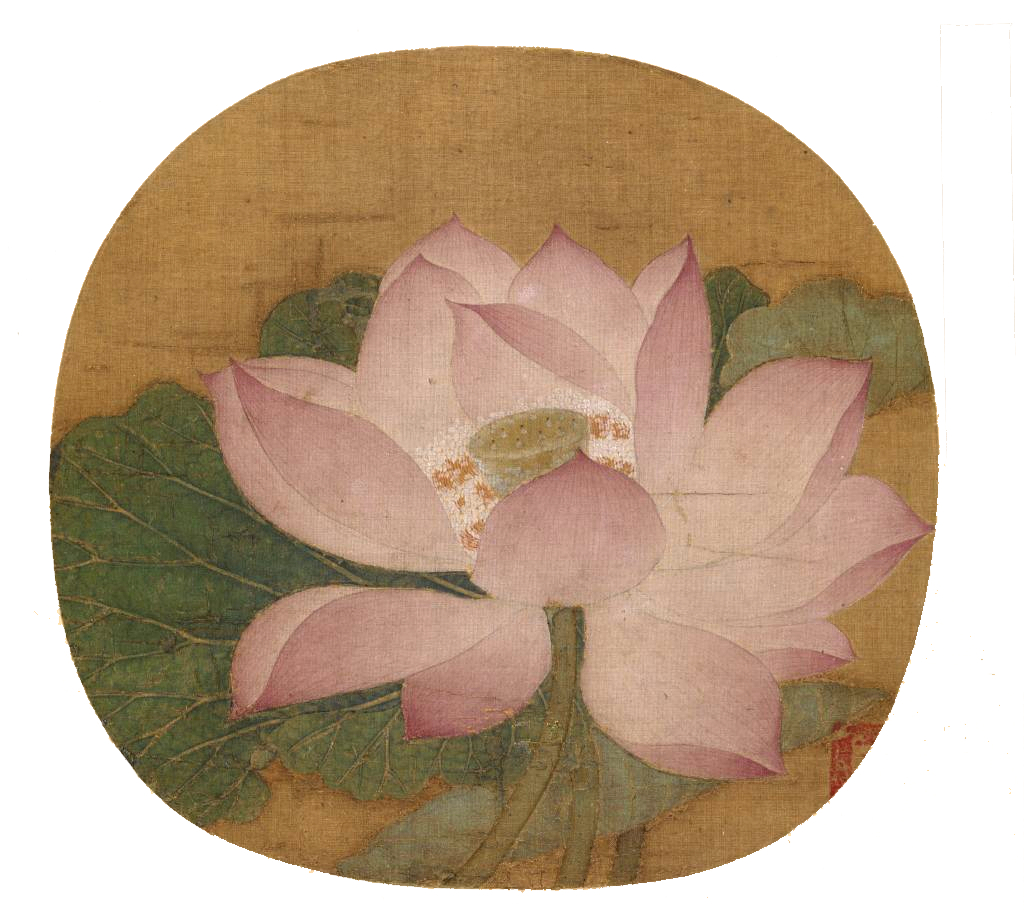
\includegraphics[width=1.5cm]{../pics/S.jpg}};
    \node at ($(S)+(0,-1)$) (S_text) {$S$};
    

    %创建一个神经网络, 用于表示Dsal模块, 并定义一个Dasl坐标表示这个模块
    \coordinate (Dsal) at ($(S)+(\offX,0)$);
    \networkLayer{1.5}{0.15}{0.0}{0.0}{0.0}{color=GanYu_midblue!40}{}{start}{(0,0,0)};
    \networkLayer{1}{0.15}{0.1}{0.0}{0.0}{color=GanYu_midblue!50}{}{}{(0,0,0)};
    \networkLayer{0.75}{0.15}{0.1}{0.0}{0.0}{color=GanYu_midblue!70}{}{mid_right}{(0,0,0)};
    \networkLayer{1}{0.15}{0.2}{0.0}{0.0}{color=GanYu_midblue!40}{}{last}{(0,0,0)};
    \node at ($(mid_right_bottom)+(-0.08,-0.7)$) (Dsal_bottom) {$D_{sal}$};

    %创建一个方形, 用于表示Msal, 是一个矩阵
    \coordinate (Msal) at ($(Dsal)+(\offX,0)$);
    \def\widthMsal{1.2};
    \coordinate (Msal_left_bottom) at ($(Msal)+(-\widthMsal/2,-\widthMsal/2)$);
    \coordinate (Msal_right_bottom) at ($(Msal)+(\widthMsal/2,\widthMsal/2)$);
    \coordinate (Msal_left) at ($(Msal)+(-\widthMsal/2-0.1,0)$);
    \coordinate (Msal_right) at ($(Msal)+(\widthMsal/2+0.1,0)$);
    \coordinate (Msal_upper) at ($(Msal)+(0,\widthMsal/2+0.1)$);
    \coordinate (Msal_bottom) at ($(Msal)+(0,-\widthMsal/2-0.1)$);
    \draw (Msal_left_bottom) rectangle (Msal_right_bottom);
    \node at ($(Msal)+(0,-\widthMsal/2-0.5)$) (Msal_text) {$M_{sal}$};
    %为Msal的方格涂上颜色
    \fill[black!80] ($(Msal_left_bottom)+(\widthMsal/3*0, \widthMsal/3*0)$) rectangle ($(Msal_left_bottom)+(\widthMsal/3*0+\widthMsal/3, \widthMsal/3*0+\widthMsal/3)$);
    \fill[black!85] ($(Msal_left_bottom)+(\widthMsal/3*0, \widthMsal/3*1)$) rectangle ($(Msal_left_bottom)+(\widthMsal/3*0+\widthMsal/3, \widthMsal/3*1+\widthMsal/3)$);
    \fill[black!90] ($(Msal_left_bottom)+(\widthMsal/3*2, \widthMsal/3*1)$) rectangle ($(Msal_left_bottom)+(\widthMsal/3*2+\widthMsal/3, \widthMsal/3*1+\widthMsal/3)$);
    \fill[black!90] ($(Msal_left_bottom)+(\widthMsal/3*1, \widthMsal/3*2)$) rectangle ($(Msal_left_bottom)+(\widthMsal/3*1+\widthMsal/3, \widthMsal/3*2+\widthMsal/3)$);
    \fill[lightgray] ($(Msal_left_bottom)+(\widthMsal/3*0, \widthMsal/3*2)$) rectangle ($(Msal_left_bottom)+(\widthMsal/3*0+\widthMsal/3, \widthMsal/3*2+\widthMsal/3)$);
    \fill[lightgray] ($(Msal_left_bottom)+(\widthMsal/3*1, \widthMsal/3*0)$) rectangle ($(Msal_left_bottom)+(\widthMsal/3*1+\widthMsal/3, \widthMsal/3*0+\widthMsal/3)$);
    \fill[lightgray] ($(Msal_left_bottom)+(\widthMsal/3*1, \widthMsal/3*1)$) rectangle ($(Msal_left_bottom)+(\widthMsal/3*1+\widthMsal/3, \widthMsal/3*1+\widthMsal/3)$);
    \fill[lightgray] ($(Msal_left_bottom)+(\widthMsal/3*2, \widthMsal/3*0)$) rectangle ($(Msal_left_bottom)+(\widthMsal/3*2+\widthMsal/3, \widthMsal/3*0+\widthMsal/3)$);
    \fill[lightgray] ($(Msal_left_bottom)+(\widthMsal/3*2, \widthMsal/3*2)$) rectangle ($(Msal_left_bottom)+(\widthMsal/3*2+\widthMsal/3, \widthMsal/3*2+\widthMsal/3)$);
    % 为Msal划上方格, 表示一个矩阵
    \foreach \y in {0, \widthMsal/3, 2*\widthMsal/3}{
        \draw[black,thin] ($(Msal_left_bottom)+(0,\y)$) -- ($(Msal_left_bottom)+(\widthMsal,\y)$);
    }
    \foreach \x in {0, \widthMsal/3, 2*\widthMsal/3}{
        \draw[black, thin] ($(Msal_left_bottom)+(\x,0)$) -- ($(Msal_left_bottom)+(\x,\widthMsal)$);
    }

    % 创建一个\odot符号
    \coordinate (odot1) at ($(Msal)+(\offX-0.5,0)$);
    \node at (odot1) (odot1) {\large $\odot$};

    % 创建一个用于表示风格主体图像Sm的node
    \coordinate (Sm) at ($(odot1)+(\offX,0)$);
    \node at (Sm) (Sm_fig) {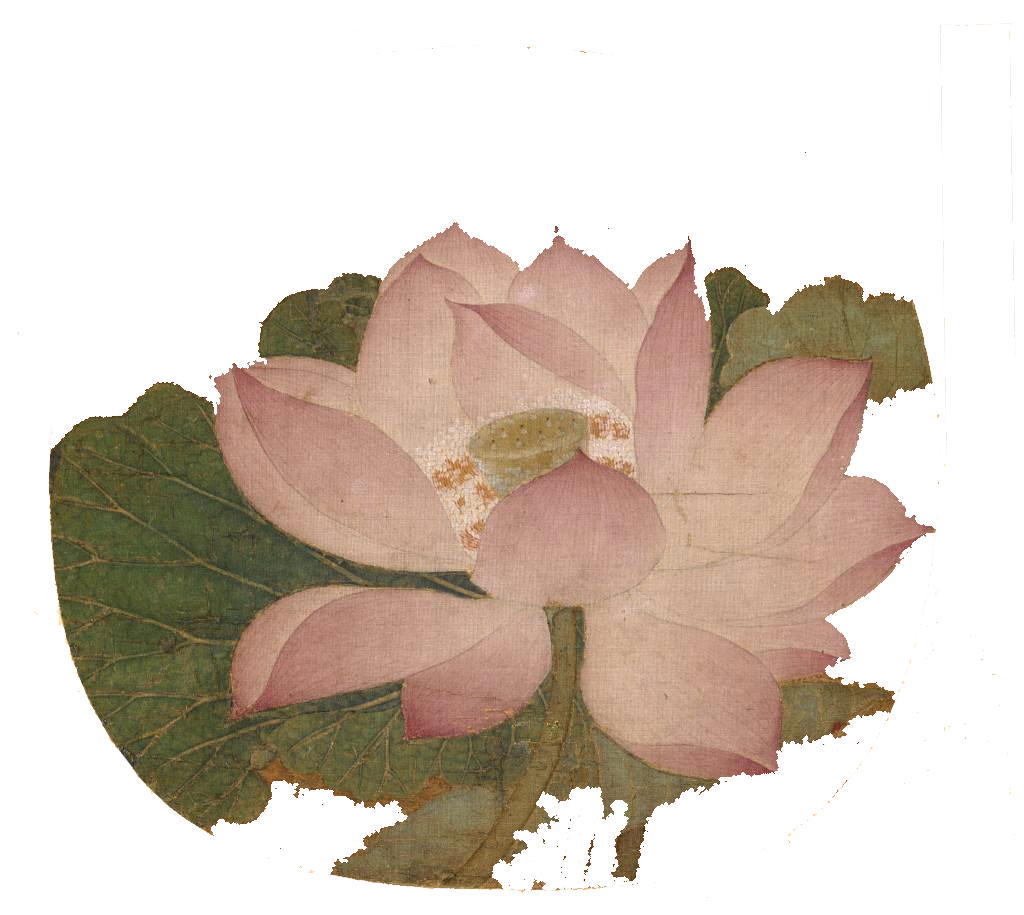
\includegraphics[width=1.5cm]{../pics/S_m.jpg}};
    \node at ($(Sm)+(0,-1)$) (Sm_text) {$S_m$};

    %创建一个方形, 用于表示I-Msal模块
    \coordinate (IMsal) at ($(Dsal)+(0,-\offY)$);
    \def\widthIMsal{1.2};
    \coordinate (IMsal_left_bottom) at ($(IMsal)+(-\widthIMsal/2,-\widthIMsal/2)$);
    \coordinate (IMsal_right_bottom) at ($(IMsal)+(\widthIMsal/2,\widthIMsal/2)$);
    \coordinate (IMsal_left) at ($(IMsal)+(-\widthIMsal/2-0.1,0)$);
    \coordinate (IMsal_right) at ($(IMsal)+(\widthIMsal/2+0.1,0)$);
    \coordinate (IMsal_upper) at ($(IMsal)+(0,\widthIMsal/2+0.1)$);
    \coordinate (IMsal_bottom) at ($(IMsal)+(0,-\widthIMsal/2-0.1)$);
    \draw (IMsal_left_bottom) rectangle (IMsal_right_bottom);
    \node at ($(IMsal)+(0,-\widthIMsal/2-0.5)$) (IMsal_text) {$I-M_{sal}$};
    %为IMsal的方格涂上颜色
    \fill[black!20] ($(IMsal_left_bottom)+(\widthIMsal/3*0, \widthIMsal/3*0)$) rectangle ($(IMsal_left_bottom)+(\widthIMsal/3*0+\widthIMsal/3, \widthIMsal/3*0+\widthIMsal/3)$);
    \fill[black!15] ($(IMsal_left_bottom)+(\widthIMsal/3*0, \widthIMsal/3*1)$) rectangle ($(IMsal_left_bottom)+(\widthIMsal/3*0+\widthIMsal/3, \widthIMsal/3*1+\widthIMsal/3)$);
    \fill[darkgray] ($(IMsal_left_bottom)+(\widthIMsal/3*0, \widthIMsal/3*2)$) rectangle ($(IMsal_left_bottom)+(\widthIMsal/3*0+\widthIMsal/3, \widthIMsal/3*2+\widthIMsal/3)$);
    \fill[darkgray] ($(IMsal_left_bottom)+(\widthIMsal/3*1, \widthIMsal/3*0)$) rectangle ($(IMsal_left_bottom)+(\widthIMsal/3*1+\widthIMsal/3, \widthIMsal/3*0+\widthIMsal/3)$);
    \fill[darkgray] ($(IMsal_left_bottom)+(\widthIMsal/3*1, \widthIMsal/3*1)$) rectangle ($(IMsal_left_bottom)+(\widthIMsal/3*1+\widthIMsal/3, \widthIMsal/3*1+\widthIMsal/3)$);
    \fill[black!10] ($(IMsal_left_bottom)+(\widthIMsal/3*1, \widthIMsal/3*2)$) rectangle ($(IMsal_left_bottom)+(\widthIMsal/3*1+\widthIMsal/3, \widthIMsal/3*2+\widthIMsal/3)$);
    \fill[darkgray] ($(IMsal_left_bottom)+(\widthIMsal/3*2, \widthIMsal/3*0)$) rectangle ($(IMsal_left_bottom)+(\widthIMsal/3*2+\widthIMsal/3, \widthIMsal/3*0+\widthIMsal/3)$);
    \fill[black!10] ($(IMsal_left_bottom)+(\widthIMsal/3*2, \widthIMsal/3*1)$) rectangle ($(IMsal_left_bottom)+(\widthIMsal/3*2+\widthIMsal/3, \widthIMsal/3*1+\widthIMsal/3)$);
    \fill[darkgray] ($(IMsal_left_bottom)+(\widthIMsal/3*2, \widthIMsal/3*2)$) rectangle ($(IMsal_left_bottom)+(\widthIMsal/3*2+\widthIMsal/3, \widthIMsal/3*2+\widthIMsal/3)$);
    % 为I-Msal划上方格, 表示一个矩阵
    \foreach \y in {0, \widthMsal/3, 2*\widthMsal/3}{
        \draw[black, thin] ($(IMsal_left_bottom)+(0,\y)$) -- ($(IMsal_left_bottom)+(\widthIMsal,\y)$);
    }
    \foreach \x in {0, \widthIMsal/3, 2*\widthIMsal/3}{
        \draw[black, thin] ($(IMsal_left_bottom)+(\x,0)$) -- ($(IMsal_left_bottom)+(\x,\widthIMsal)$);
    }

    % 创建一个\odot符号
    \coordinate (odot2) at ($(IMsal)+(\offX-0.5,0)$);
    \node at (odot2) (odot2) {\large $\odot$};

    % 创建一个用于表示风格主体图像Sb的node
    \coordinate (Sb) at ($(odot2)+(\offX,0)$);
    \node at (Sb) (Sb_fig) {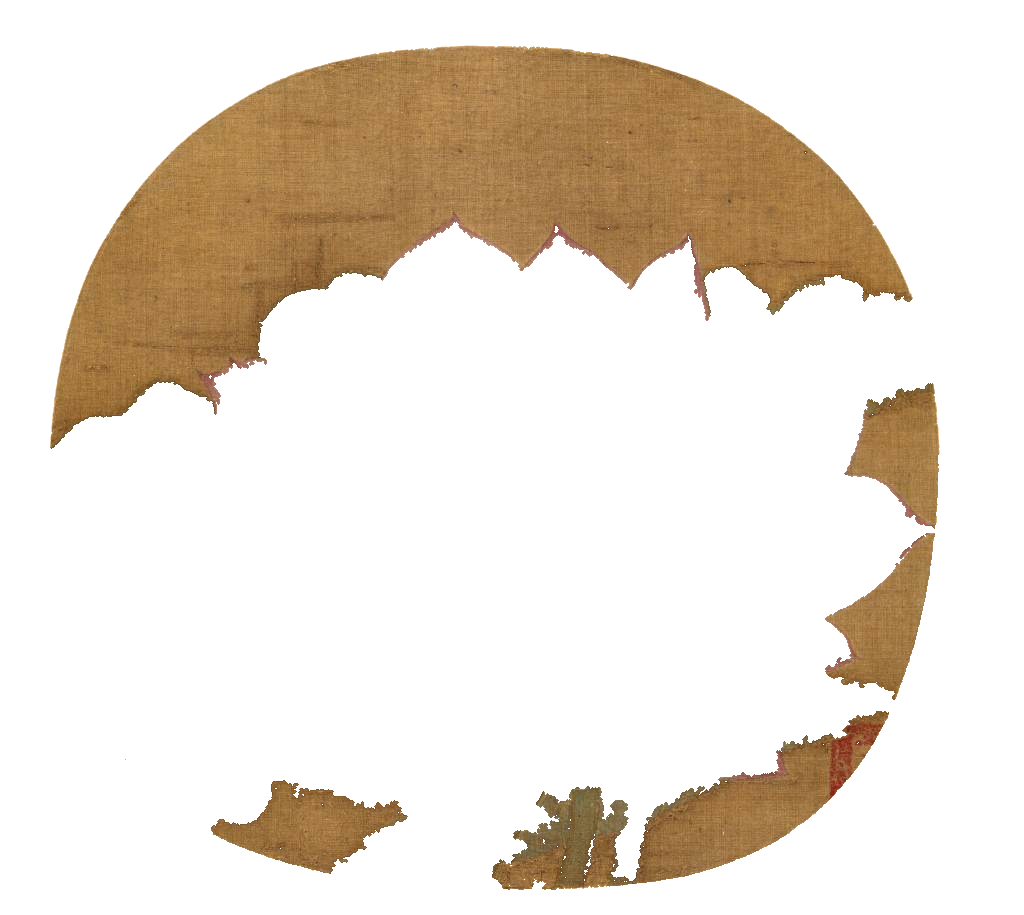
\includegraphics[width=1.5cm]{../pics/S_b.jpg}};
    \node at ($(Sb)+(0,-1)$) (Sb_text) {$S_b$};


    % 绘制箭头
    % S上的出度箭头1:S->Dsal
    \draw[->, thick] (S_fig.east) -- ($(start_back)+(-0.5,0)$);
    % S上的出度箭头2:S -> odot1
    \draw[->, thick] (S_fig.north)  -- ($(S)+(0,1.5)$) -| (odot1.north);
    % S上的出度箭头3:S -> IMsal
    \draw[->, thick] (S_text.south) -- ($(S)+(0,-4.5)$)  -| (odot2.south);

    % Dsal的出度箭头1:Dsal->Msal
    \draw[->, thick] ($(last_front)+(0.3,0)$) -- (Msal_left);
    % Dsal的出度箭头2:Dsal->I-Msal
    \draw[->, thick] (Dsal_bottom.south) -- (IMsal_upper);

    % Msal的出度箭头箭头1:Msal->odot
    \draw[->, thick] (Msal_right) -- (odot1.west);

    % odot1的出度箭头1:odot1->Sm
    \draw[->, thick] (odot1.east) -- (Sm_fig.west);

    % IMsal的出度箭头1:IMsal->odot2
    \draw[->, thick] (IMsal_right) -- (odot2.west);
    
    % odot2的出度箭头1:odot2->Sb
    \draw[->, thick] (odot2.east) -- (Sb_fig.west);
    
    % \networkLayer{3.0}{0.1}{0.5}{0.0}{0.0}{color=white}{conv}{}{};
    % Use the new command to draw a set of rounded rectangles
    % \rSquare{1}{NekasuBlue}{70}{5pt}{0}{0};
    % \rSquare{1}{NekasuBlue}{70}{5pt}{-0.5}{-0.5};
    % \rSquare{1}{NekasuBlue}{70}{5pt}{-1}{-1};
    % \rSquareSet{1}{NekasuBlue}{70}{5pt}{0}{0}{0.2}{ExampleSet}{0.5};
    % \draw[->,thick] ($(ExampleSet_left) + (-2,0)$) -- (ExampleSet_left);
\end{tikzpicture}

\end{document}
